\section{Introduction}
In today's age of information and connectivity, advances in Artificial Intelligence (AI) and Machine Learning (ML) have transformed the way users interact with technology and process data.

Among the emerging paradigms in the field of ML, Federated Learning (FL) appeared as an innovative approach to train AI models in a distributed and decentralized environment.

In the last decade, ML has revolutionized the way in which we face complex problems in different areas, from computer vision to natural language processing. The last two years have been filled with news about promising new paradigms of image generation, classification, chatbots, speech recognition and other AI's and, as time goes by, the applications of AI are becoming more present in our daily lives.

We can find examples of applications using FL in examples such as the text predictive keyboard that we can find on our mobile phones (Google's Android Keyboard \cite{GoogleKeyboard}). We also find FL in Apple's assistant Siri voice recognition. This technology  helps distinguish whether it is the main user of the smartphone saying "Hey, Siri", or another iPhone user attempting to activate Siri on their phone. As a final example, FL is used in more complex applications such as autonomous driving systems. In all three cases, the use of FL allows the machine learning models to be trained with the users' data without them having to share their data with third parties. In the case of Google's predictive keyboard, the model is trained with the users' data locally on the device, while in the case of the autonomous driving systems, the users' data is used to train the model in a distributed way among the vehicles in the fleet.

Despite its advantages in terms of privacy, scalability and efficiency, FL presents significant challenges. One of them is its vulnerability to attacks: these attacks can exploit the distributed nature of the learning process, aiming to compromise integrity, confidentiality, and the model's efficiency. As seen in the real-world examples, if an attacker exploited a vulnerability of the autonomous driving system by modifying the action that the car takes when recognising a STOP sign, changing it to the action taken when recognising 120km/h sign, causing the vehicle to accelerate at full capacity, it could lead to multiple car accidents. In the context of FL this is known as a label flipping attack.

As Federated Learning systems are increasingly integrated in real-world applications, it becomes necessary to understand and address these challenges to guarantee a successful and secure deployment of this technology.


%The GitHub repository "LFighter" \cite{LFighter_code} by Najeeb Jabreel is this thesis inspiration. It already offers a working FL simulator, where the programmer can modify the environment's parameters and obtain results of attacks against a variety of servers with different rules. With the explicit purpose of formulating and deploying attacks against FL systems to assess their robustness, this simulator serves as the foundation for the development of this thesis.



\subsection{Motivation}
Since the paper proposing FL got published in 2017, this new paradigm has been increasingly used over the years as we can see in \autoref{fig:popularity_FL}.
With its increase in popularity and, its implementation in sensitive applications such as autonomous driving systems, our concerns about the security of this technology also increase.

From this concern, the motivation of detecting possible vulnerabilities so they can be addressed arises. 

\begin{figure}[h!]
        % \begin{figure}[H] % Alternative positioning
        \centering % sempre
        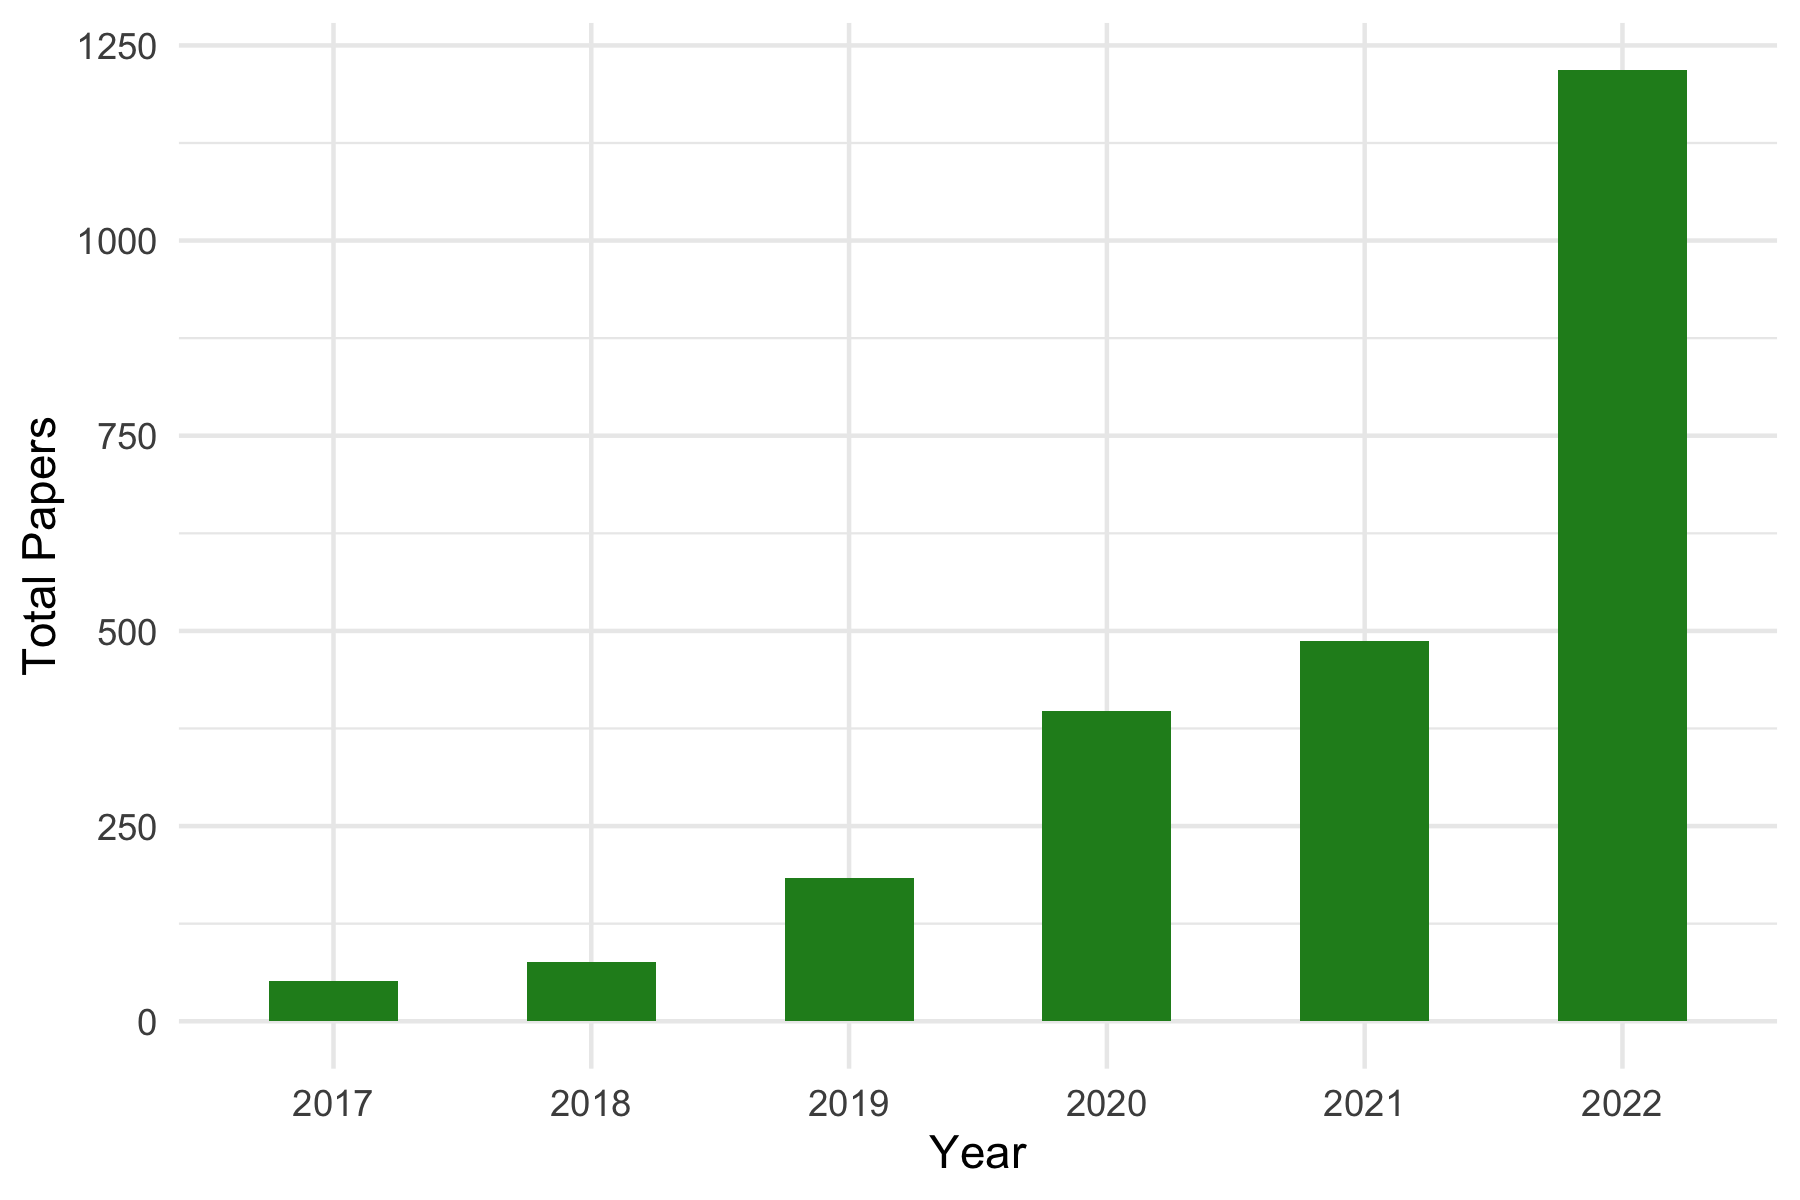
\includegraphics[scale=0.2]{popularity_FL.png}
        \caption{Published papers per year since FL was proposed. Source: \textit{Web of Science}} % sempre
        \label{fig:popularity_FL}
    \end{figure}

\subsection{Objectives}
The main theoretical objective of this thesis is to explore and examine in detail the kind of attacks that can be directed towards Federated Learning systems, as well as identifying strategies and solutions to mitigate these attacks. 

The practical objective is to examine the effectiveness and implications of employing a sophisticated label flipping technique compared to a straightforward approach when targeting a Federated Learning system. Specifically, the focus is on evaluating whether a more strategic and intelligent choice of samples to suffer a label flipping can lead to greater success for potential attackers compared to indiscriminately flipping all labels. This investigation represents an essential step towards comprehending the vulnerabilities and potential weak points within the Federated Learning paradigm. Furthermore, we aim to provide results on some of the most used aggregation rules in Federated Learning systems.

The research may be able to identify patterns and insights that conventional methods of attack might miss by examining the results of strategically manipulated label flipping and comparing them with the brute-force method.
The results of this thesis will be valuable in gaining a deeper understanding of the security implications of FL and to develop more robust and secure FL systems in case the conceived attacks succeed.


In summary, this thesis conducts a critical examination of the viability of using intelligent label flipping techniques in comparison to a brute-force approach when attacking a Federated Learning system.

\subsection{Outline}
The remainder of this thesis organized in the following sections:
\begin{itemize}
    \item Section \ref{sec:background}, Background: Provides a brief overview of the Federated Learning paradigm, its advantages and disadvantages, and the different types of attacks that can be directed towards it.
    \item Section \ref{sec:design_attacks}, Design of the proposed attacks: It describes the different attack hypotheses that are proposed.
    \item Section \ref{sec:architecture}, Implementation: Explains the implementation of the new code.
    \item Section \ref{sec:results}, Results: Presents the results obtained from the experiments conducted with the new code.
    \item Section \ref{sec:conclusions}, Conclusions: Summarizes the conclusions drawn from the results obtained in the experiments.
\end{itemize}

\pagebreak